\documentclass{fm}

\usepackage[utf8]{inputenc}  
\usepackage[ngerman]{babel}
\usepackage{pdfpages}

\begin{document}
\Abgabeblatt{1}{Do 26.05.2011}{}{Gruppe:}{Philipp Dittmann}{Patrick Fehrmann}{}
\section*{Übung 1}
Es galt ein Banksystem zu schreiben, welches die Kriterien von \glqq{}exercise01.pdf\grqq{} (auf Stud.IP downloadbar) erfüllt. Dieses Banksystem soll gängige Geldtransferabläufe simulieren (Einzahlung, Auszahlung, Überweisung, ...). Dabei sind eine Bank und mehrere Personen involviert. Es gibt Einzelkonten und Gemeinschaftskonten, die getrennt abgearbeitet werden mussten. Es sollte darauf geachtet werden, dass im System kein Geld verloren geht und keine Grenzen überschritten werden (Konto überziehen, zu viele Kredite, etc.).

Das ganze wurde zusätzlich mit JML beschrieben, um den Quellcode statisch auswerten zu lassen.

Anbei befindet sich noch eine kleine Vererbungshierarchie, um sich besser zurechtzufinden. Der Quellcode liegt als ZIP gepackt dabei.
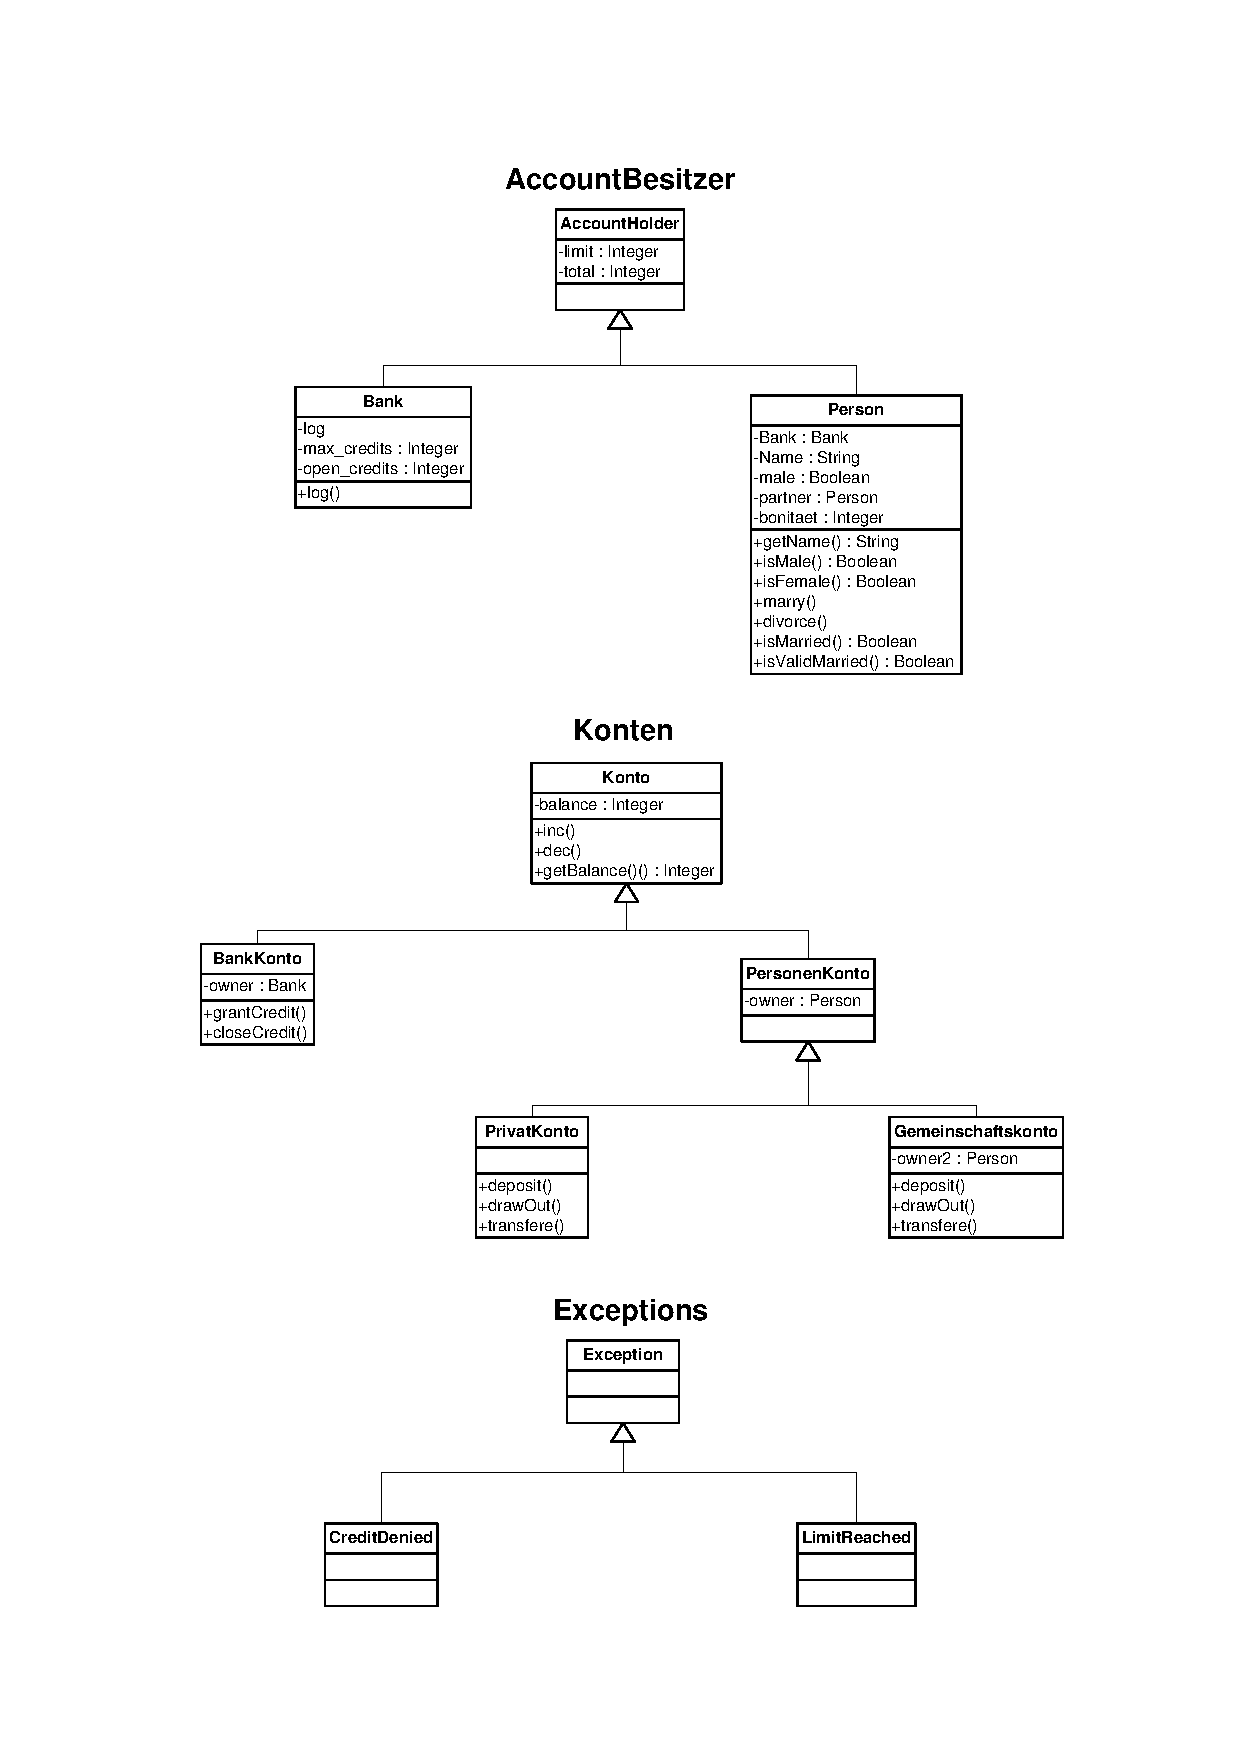
\includepdf[pages=-]{JML.pdf}
\end{document}